\documentclass[]{article}
\usepackage{geometry,tikz,lipsum,amsmath,amssymb,mathrsfs,soul,xcolor,cancel,esint,graphicx}
\tikzset{every picture/.style={line width=0.75pt}} %set default line width to 0.75pt        
\numberwithin{equation}{section}

\NewDocumentCommand{\caja}{ m O{gray!40} O{gray!10} m }{
	\begin{figure}[h]
		\centering
		\begin{tikzpicture}
			\node[anchor=text, text width=\columnwidth-1.2cm, draw, rounded corners, line width=1pt, fill=#3, inner sep=5mm] (big) {\\#4};
			\node[draw, rounded corners, line width=.5pt, fill=#2, anchor=west, xshift=5mm] (small) at (big.north west) {#1};
		\end{tikzpicture}
	\end{figure}
}
\NewDocumentCommand{\indUpDown}{ O{\Lambda} O{\mu} O{\nu} }{
	{#1}^{#2}_{\ #3}
}
\NewDocumentCommand{\indDownUp}{ O{\Lambda} O{\mu} O{\nu} }{
	{#1}_{#2}^{\ #3}
}
\newcommand{\LambdaMuNu}{\indUpDown}
\newcommand{\0}{\textcolor{gray}{0}}
\newcommand{\rbf}{\mathbf{r}}
\newcommand{\ei}{\mathbf{e}_i}
\newcommand{\ej}{\mathbf{e}_j}
\newcommand{\lc}{\epsilon_{ijk}}

\newcommand{\deriv}[3]{\left(\frac{\partial #1}{\partial #2} \right)_{#3}}
\newcommand{\dderiv}[3]{\left(\dfrac{\partial #1}{\partial #2} \right)_{#3}}

\newcommand{\qed}{\hfill\(\blacksquare\)}

%opening
\title{Tarea 1 Mecánica Estadística Avanzada}
\author{Simon Fonseca}

\begin{document}
\maketitle

Como primera tarea les corresponde realizar 10 de los 21 problemas 1-23, 1-24, 1-27, 1-28, 1-30, 2-13, 2-15, 2-16, 2-17, 2-19, 3-4, 3-5, 3-7, 3-8, 3-9, 3-17, 3-19, 3-20, 3-22, 3-23, 3-24 del libro de Mc. Quarrie.

\section{Problema 1.23}
Verify the calculation:
\begin{equation}
	\Omega(E, \Delta E)=\frac{1}{\Gamma(N+1) \Gamma(3 N / 2)}\left(\frac{2 \pi m a^2}{h^2}\right)^{3 N / 2} E^{(3 N / 2-1)} \Delta E
\end{equation}
In this case, $E=3 N k T / 2$. If we take $T=300^{\circ} \mathrm{K}, m=10^{-22} \mathrm{~g}, a=10 \mathrm{~cm}$, $N=6.02 \times 10^{23}$, and $\Delta E$ equal to $0.01 E$, we get $\Omega(E, \Delta E)$ to be $O\left(10^N\right)$.
\\

\textbf{Respuesta:}
Resumiendo los valores dados:
\begin{equation}
	\left\lbrace \begin{matrix}
		E &=& 3 N k T / 2\\
		T &=& 300 \mathrm{~K}\\
		m &=& 10^{-22} \mathrm{~g} &=& 10^{-25} \mathrm{~kg} \\
		a &=& 10 \mathrm{~cm} &=& 0.1 \mathrm{~m}\\
		N &=& 6.02 \times 10^{23}\\
		\Delta E &=& 0.01 E &=& E/100
	\end{matrix}\right. 
\end{equation}
Luego,
\begin{align*}
	\Omega(E, \Delta E) &= \frac{1}{\Gamma(N+1) \Gamma(3 N / 2)}\left(\frac{2 \pi m a^2}{h^2}\right)^{3 N / 2} \frac{E^{(3 N / 2-1)}\cdot E}{100}\\
	&= \frac{1}{100}\frac{1}{\Gamma(N+1) \Gamma(3 N / 2)}\left(1.43109\times 10^{40} E\right)^{3 N / 2}\\
	&= \frac{1}{100}\frac{1}{\Gamma(N+1) \Gamma(3 N / 2)}\left(8.38389\times 10^{29} \right)^{N}N^{3N/2}
\end{align*}
Usando la aproximación de Stirling:
\begin{equation}
	\Gamma(x + 1) \approx \sqrt{2\pi x}\left(\frac{x}{e}\right)^{x}
\end{equation}
\begin{align*}
	\Rightarrow \Gamma(N+1) \Gamma(3 N / 2) &\approx 2\pi \sqrt{N}\sqrt{3N/2 - 1} \left(\frac{N}{e}\right)^{N} \left(\frac{3N/2 - 1}{e}\right)^{3N/2 - 1}
\end{align*}
Pero \(3N/2 - 1\approx 3N/2\), entonces
\begin{align*}
	\Rightarrow \Gamma(N+1) \Gamma(3 N / 2) &\approx 2\pi \sqrt{N}\sqrt{3N/2} \left(\frac{N}{e}\right)^{N} \left(\frac{3N/2 - 1}{e}\right)^{3N/2 - 1}\\
	&\approx \sqrt{6}\pi\frac{N^{N + 1} (3N/2)^{3N/2}}{e^{5N/2}}\frac{2e}{3N}\\
	&\approx \frac{2\sqrt{6}\pi e}{3}\frac{3^{3N/2}}{2^{3N/2}e^{5N/2}}N^{N} N^{3N/2}\\
	&\approx \frac{2\sqrt{6}\pi e}{3}\left( \frac{3^{3}}{2^{3}e^{5}}\right)^{N/2}N^{5N/2}\\
	&\approx \frac{2\sqrt{6}\pi e}{3}\left(0.1508\right)^{N}N^{5N/2}
\end{align*}
Luego
\begin{align*}
	\Omega(E, \Delta E) &\approx \frac{1}{100}\frac{3}{2\sqrt{6}\pi e\left(0.1508\right)^{N}N^{5N/2}} \left(8.38389\times 10^{29} \right)^{N}N^{3N/2}\\
	&\approx \underbrace{\frac{3}{200\sqrt{6}\pi e}}_{\approx 0}\left(5.55962\times 10^{30} \right)^{N}N^{-N}\\
	&\approx \left(\frac{5.55962\times 10^{30}}{N} \right)^{N}\\
	&\approx \left(9.23524\times 10^6 \right)^{N}  \propto 10^{6N}
\end{align*}
Pero \(6N \propto N\), entonces
\begin{equation}
	\Omega(E, \Delta E) \propto 10^{N}
\end{equation}
\qed

% % % % % % % % % % % % % % % % % % % % % % % % % % % % % % % % % % % % % % % % % % % % % % % % % % % % % %

\section{Problema 1.24}
We need to know the volume of an $N$-dimensional sphere in order to derive Eq. (1-36). This can be determined by the following device. Consider the integral
\begin{equation}
	I=\int_{-\infty}^{\infty} \int e^{-\left(x_1^2+x_2^2+\cdots+x_N^2\right)} d x_1 d x_2 \cdots d x_N
	\label{1.24_I}
\end{equation}

\begin{enumerate}
	\item[a.] First show that $I = \pi^{N / 2}$.
	\\
	
	\textbf{Respuesta:}
	De la ec. \ref{1.24_I}
	\begin{align}
		I &= \int_{-\infty}^{\infty} \int e^{-\left(x_1^2+x_2^2+\cdots+x_N^2\right)} d x_1 d x_2 \cdots d x_N\nonumber\\
		&= \int_{-\infty}^{\infty} \int e^{-x_1^2}e^{-x_2^2}\cdots e^{-x_N^2} d x_1 d x_2 \cdots d x_N\nonumber\\
		&= \left(\int_{-\infty}^{\infty}e^{-x^2}dx\right)^N\nonumber\\
		&= \left(\sqrt{\pi}\right)^N = \pi^{N/2}\label{1.24_I_pi}
	\end{align}
	\qed

	\item[b.] Now one can formally transform the volume element $d x_1 d x_2 \cdots d x_N$ to $N$-dimensional spherical (hyperspherical) coordinates to get
	\begin{equation}
		\int_{\text {angles }} d x_1 d x_2 \cdots d x_N \rightarrow r^{N-1} S_N d r
	\end{equation}
	where $S_N$ is the factor that arises upon integration over the angles. Show that $S_2 = 2 \pi$ and $S_3=4 \pi$.
	\\
	
	\textbf{Respuesta:}
	Para \(N=2\)
	\begin{equation}
		\iint_{\text {angles }} dx_1 dx_2 \label{1.24_N2}
	\end{equation}
	De donde podemos identificar \(dx_1, dx_2\) con las coordenadas polares:
	\begin{alignat*}{2}
		dx_1 &= dr&&\left\lbrace \begin{matrix}
			r_\text{i} &=& 0\\
			r_\text{f} &=& R
		\end{matrix}\right. \\
		dx_2 &= r d\theta &&\left\lbrace \begin{matrix}
			\theta_\text{i} &=& 0\\
			\theta_\text{f} &=& 2\pi
		\end{matrix}\right. 
	\end{alignat*}
	Luego, ec. \ref{1.24_N2}
	\begin{align}
		\iint_{\text {angles }} dx_1 dx_2 &= \iint_{0}^{2\pi} r d\theta dr\nonumber\\
		&= \int \underbrace{2\pi}_{S_2} \cdot \underbrace{r}_{r^{N-1}} dr
	\end{align}
	\qed
	
	Para \(N=3\)
	\begin{equation}
		\iiint_{\text {angles }} dx_1 dx_2 dx_3 \label{1.24_N3}
	\end{equation}
	De donde podemos identificar \(dx_1, dx_2, dx_3\) con las coordenadas esféricas:
	\begin{alignat*}{2}
		dx_1 &= dr&&\left\lbrace \begin{matrix}
			r_\text{i} &=& 0\\
			r_\text{f} &=& R
		\end{matrix}\right. \\
		dx_2 &= r d\theta &&\left\lbrace \begin{matrix}
			\theta_\text{i} &=& 0\\
			\theta_\text{f} &=& \pi
		\end{matrix}\right. \\
		dx_3 &= r \sin \theta d\varphi &&\left\lbrace \begin{matrix}
		\varphi_\text{i} &=& 0\\
		\varphi_\text{f} &=& 2\pi
		\end{matrix}\right.
	\end{alignat*}
	Luego, ec. \ref{1.24_N3}
	\begin{align}
		\iiint_{\text {angles }} dx_1 dx_2 &= \iint_{0}^{2\pi}\int_{0}^{\pi} r \cdot r \sin \theta d\theta d\varphi dr\nonumber\\
		&= \iint_{0}^{2\pi} 2 r^2  d\varphi dr\nonumber\\
		&= \int \underbrace{4\pi}_{S_3} \cdot \underbrace{r^2}_{r^{N-1}} dr
	\end{align}
	\qed
	
	\item[c.] $S_N$ can be determined for any $N$ by writing $I$ in hyperspherical coordinates:
	\begin{equation}
		I = \int_0^{\infty} e^{-r^2} r^{N-1} S_N d r \label{1.24_I_hyper}
	\end{equation}
	
	Show that $I=S_N \Gamma(N / 2) / 2$, where $\Gamma(x)$ is the gamma function (see Problem 1-58).
	\\
	
	\textbf{Respuesta:}
	La definición de la función Gamma:
	\begin{equation}
		\Gamma(z) = \int_0^{\infty}x^{z-1} e^{-x} dx\label{Gamma}
	\end{equation}
	El cuál, para cualquier entero positivo \(n\), es igual a
	\begin{equation}
		\Gamma(n) = (n - 1)!\label{Gamma_factorial}
	\end{equation}
	Y tiene la propiedad fundamental:
	\begin{equation}
		\Gamma(z + 1) = z \Gamma(z)\label{Gamma_propiedad}
	\end{equation}
	De la ec. \ref{1.24_I_hyper}:
	\begin{align*}
		I &= S_N \int_0^{\infty} r^{N-1} e^{-r^2} d r
	\end{align*}
	Con el cambio de variables:
	\begin{equation*}
		u \equiv r^2,\ \ \ du = 2 r d r
	\end{equation*}
	Obtenemos:
	\begin{align}
		I &= S_N \int_0^{\infty} u^{\frac{N-1}{2}} e^{-u} d r\nonumber\\
		&= S_N \int_0^{\infty} u^{N/2 - 1}\sqrt{u}\cdot e^{-u} d r\nonumber\\
		&= S_N \frac{1}{2} \int_0^{\infty} u^{N/2 - 1}\cdot e^{-u} \underbrace{2 r d r}_{du}\nonumber\\
		&= \frac{S_N}{2} \int_0^{\infty} u^{N/2 - 1} e^{-u} du\nonumber\\
		I &= \frac{S_N}{2} \Gamma(N / 2)\label{1.24_I_Gamma}
	\end{align}
	\qed
	
	\item[d.] Equate these two values (eqs. \ref{1.24_I_pi} and \ref{1.24_I_Gamma}) for $I$ to get
	\begin{equation}
		S_N = \frac{2 \pi^{N / 2}}{\Gamma(N / 2)}
	\end{equation}
	
	\textbf{Respuesta:}
	Tomando las ecs. \ref{1.24_I_pi} y \ref{1.24_I_Gamma}:
	\begin{align*}
		I = \pi^{N/2} &= \frac{S_N}{2} \Gamma(N / 2)\\
		\Rightarrow S_N &= \frac{2 \pi^{N/2}}{\Gamma(N / 2)}
	\end{align*}
	\qed
	
	\item[e.] Show that this reduces correctly for $N=2$ and 3.
	\\
	
	\textbf{Respuesta:}
	Para \(N=2\):
	\begin{align*}
		S_2 &= \frac{2 \pi^{2/2}}{\Gamma(2 / 2)}\\
		&= \frac{2\pi}{\Gamma(1)} = \frac{2\pi}{0!}\\
		&= 2\pi
	\end{align*}
	\qed
	
	Para \(N=3\), y considerando que \(\Gamma(3/2) = \sqrt{\pi}/2\):
	\begin{align*}
		S_3 &= \frac{2 \pi^{3/2}}{\Gamma(3 / 2)}\\
		&= \frac{2 \pi^{3/2}}{\pi^{1/2}/2}\\
		&= 4\pi
	\end{align*}
	\qed
	
	\item[f.] Lastly now, convince yourself that the volume of an $N$-dimensional sphere of radius $a$ is given by
	\begin{equation*}
		V_N = \int_0^a S_N r^{N-1} d r=\frac{\pi^{N / 2}}{\Gamma\left(\frac{N}{2}+1\right)} a^N
	\end{equation*}
	and show that this reduces correctly for $N=2$ and 3.
	\\
	
	\textbf{Respuesta:}
	Tomando
	\begin{align*}
		V_N &= \int_0^a S_N r^{N-1} d r\\
		&= S_N \int_0^a r^{N-1} d r\\
		&= \frac{2 \pi^{N/2}}{\Gamma(N / 2)} \left[\frac{r^N}{N} \right]^{a}_{0}\\
		&= \frac{2 \pi^{N/2}}{\Gamma(N / 2)} \frac{a^N}{N}
	\end{align*}
	Pero, usando la propiedad \ref{Gamma_propiedad}, \(\Gamma\left( \frac{N}{2} + 1\right) =  \frac{N}{2} \Gamma\left(\frac{N}{2}\right)\), obtenemos
	\begin{align*}
		V_N &=  \pi^{N/2}a^N\frac{2}{N\Gamma(N / 2)}\\
		&= \frac{\pi^{N/2}}{\Gamma(N / 2 + 1)}a^N
	\end{align*}
	\qed
\end{enumerate}

% % % % % % % % % % % % % % % % % % % % % % % % % % % % % % % % % % % % % % % % % % % % % % % % % % % % % %
\section{Problema 1.27}
Show for an isothermal process that \(w_\text{rev} > w_\text{irrev}\) and \(q_\text{rev} > q_\text{irrev}\).
\\

\textbf{Respuesta:} 
De la Primera Ley de la Termodinámica:
\begin{equation}
	dE = \delta Q - \delta W \label{1ley}
\end{equation}
Y la Segunda Ley de la Termodinámica
\begin{equation}
	\delta Q \leq \frac{dS}{T} \label{2ley}
\end{equation}
Con la igualdad valiendo \textbf{solo} para procesos reversibles. Obtenemos
\begin{align*}
	\delta W &= \delta Q - dE\\
	\delta W &\leq \frac{dS}{T} - dE
\end{align*}
Ahora, para los casos reversibles e irreversibles:
\begin{equation*}
	\begin{matrix}
		\delta W_{\mathrm{rev}}   &=&    \dfrac{dS}{T} - dE\vspace{3mm}\\
		\delta W_{\mathrm{irrev}} &<& \dfrac{dS}{T} - dE
	\end{matrix}
\end{equation*}
Luego
\begin{equation*}
	\delta W_{\mathrm{rev}} > \delta W_{\mathrm{irrev}}
\end{equation*}
\qed

Además, . \ref{2ley}
\begin{equation*}
	\begin{matrix}
		\delta Q_{\mathrm{rev}} &=& \dfrac{dS}{T} \vspace{3mm}\\
		\delta Q_{\mathrm{irrev}} &<& \dfrac{dS}{T}
	\end{matrix}
\end{equation*}
Then,
\begin{equation*}
	\delta Q_{\mathrm{rev}} > \delta Q_{\mathrm{irrev}}
\end{equation*}
\qed

% % % % % % % % % % % % % % % % % % % % % % % % % % % % % % % % % % % % % % % % % % % % % % % % % % % % % %
\section{Problema 1.28}
Derive the thermodynamic equation
\begin{equation}	
	C_p - C_V = \left[p+\deriv{E}{V}{T}\right]\deriv{V}{T}{p}
\end{equation}
and evaluate this difference for an ideal gas and a gas that obeys the van der Waals equation.
\\

\textbf{Respuesta:}
Las definiciones de \(C_V\) y \(C_p\):
\begin{equation}
	\begin{matrix}
		C_V = \dderiv{E}{T}{V}, \ \ \ & 
		C_p = \dderiv{E}{T}{p} + p\dderiv{V}{T}{p}
	\end{matrix}\label{CV_Cp}
\end{equation}
Ahora, la función de estado de la energía escrita en términos de \(T,V\):
\begin{align*}
	d E &= \deriv{E}{T}{V}dT + \deriv{E}{V}{T}dV\\
	\Rightarrow \dderiv{E}{T}{p} &= \deriv{E}{T}{V} + \deriv{E}{V}{T}\deriv{V}{T}{p}\\
	&= C_V + \deriv{E}{V}{T}\deriv{V}{T}{p}
\end{align*}
Sustituyendo esto en la expresión para \(C_p\) en la ec. \ref{CV_Cp}
\begin{align}
	C_p &= C_V + \deriv{E}{V}{T}\deriv{V}{T}{p} + p\dderiv{V}{T}{p}\nonumber\\
	\Rightarrow C_p - C_V &= \left[ \deriv{E}{V}{T} + p\right] \deriv{V}{T}{p}\label{CpCV}
\end{align}
\qed

Para evaluar la ec. \ref{CpCV} para cualquier gas ideal o de Van der Waals, debemos encontrar las expresiones para
\begin{equation*}
	\deriv{E}{V}{T}\mathrm{ and }\ \deriv{V}{T}{p}
\end{equation*}
Tomando la ecuación fundamental para \(E(S,V)\):
\begin{align}
	dE &= T dS - p dV\label{fundamental_E_SV}\\
	\deriv{E}{V}{T} &= T \deriv{S}{V}{T} - p\nonumber	
\end{align}
Pero la relación de Maxwell
\begin{equation}
	\deriv{S}{V}{T} = \deriv{p}{T}{V} \label{SVT_pTV}
\end{equation}
Se convierte en
\begin{equation}
	\deriv{E}{V}{T} = T \deriv{p}{T}{V} - p\label{1.28_EVT}
\end{equation}

\vspace{4mm}
En el caso del gas ideal, tomamos la ley de los gases ideales:\vspace{2mm}
\begin{align}
	p V &= N k T \label{IdealGas}\\
	p &= \frac{N k T}{V}\nonumber
\end{align}
Obtenemos inmediatamente
\begin{align}
	V &= \frac{N k T}{p}\nonumber\\
	\Rightarrow \deriv{V}{T}{p} &= \frac{N k}{p}\label{1.28_VTp_IG}
\end{align}
Y usando ec. \ref{1.28_EVT}
\begin{align}
	\deriv{E}{V}{T} &= T \frac{N k}{V} - \frac{N k T}{V}\nonumber\\
	\deriv{E}{V}{T} &= 0\label{1.28_EVT_IG}
\end{align}
Utilizando las ecs. \ref{1.28_VTp_IG} y \ref{1.28_EVT_IG} en la ec. \ref{CpCV}
\begin{align}
	C_p - C_V &= \left[ 0 + p\right] \frac{N k}{p}\nonumber\\
	C_p - C_V &= N k
\end{align}
\qed

La ecuación de Van der Waals se define:
\begin{equation}
	p = \frac{N k T}{V - N b} - a\frac{N^2}{V^2}\label{VanDerWaals}
\end{equation}
De aquí, obtenemos
\begin{equation}
	\deriv{p}{T}{V} = \frac{N k}{V - N b}\label{pTV_VdW}
\end{equation}
Utilizando las ecs. \ref{VanDerWaals} y \ref{pTV_VdW} en la ec. \ref{1.28_EVT}
\begin{align}
	\deriv{E}{V}{T} &= T \frac{N k}{V - N b} - \left( \frac{N k T}{V - N b} - a\frac{N^2}{V^2}\right) \nonumber\\
	\deriv{E}{V}{T} &= a\frac{N^2}{V^2} \label{1.28_EVT_VdW}
\end{align}
Para la segunda derivada, reordenamos y diferenciamos la ec. \ref{VanDerWaals}
\begin{align}
	N k T &= \left( p + a\frac{N^2}{V^2}\right) \left( V - N b\right)\nonumber \\
	\Rightarrow N k &= \frac{\partial}{\partial T}\left[\left( p + a\frac{N^2}{V^2}\right) \left( V - N b\right) \right]_p\nonumber\\
	N k = \left( V - N b\right)\frac{\partial}{\partial T}&\left[\left( p + a\frac{N^2}{V^2}\right)\right]_p + \left( p + a\frac{N^2}{V^2}\right)\frac{\partial}{\partial T}\left[\left( V - N b\right) \right]_p \nonumber\\
	N k = - \left( V - N b\right)&\left(2a \frac{N^2}{V^3}\right)\deriv{V}{T}{p} + \left( p + a\frac{N^2}{V^2}\right)\deriv{V}{T}{p}\nonumber\\
	\Rightarrow \deriv{V}{T}{p} &= \dfrac{N k}{\left( p + a\dfrac{N^2}{V^2}\right) - \left( V - N b\right) \left(2a \dfrac{N^2}{V^3}\right) } \label{1.28_VTp_VdW}
\end{align}
Utilizando las ecs. \ref{1.28_EVT_VdW} y \ref{1.28_VTp_VdW} dentro de la ec. \ref{CpCV}
\begin{align*}
	C_p - C_V &= \dfrac{N k \cancel{\left(a\dfrac{N^2}{V^2} + p\right)} }{\cancel{\left( p + a\dfrac{N^2}{V^2}\right)} - \left( V - N b\right) \left(2a \dfrac{N^2}{V^3}\right) }\\
	&= \dfrac{N k}{1 - \dfrac{\left( V - N b\right) \left(2a \dfrac{N^2}{V^3}\right)}{\left(a\dfrac{N^2}{V^2} + p\right)}}
\end{align*}
Pero desde la ec. \ref{VanDerWaals} sabemos que \(a\dfrac{N^2}{V^2} + p = NkT/(V - Nb)\):
\begin{equation}
	C_p - C_V = \dfrac{N k}{1 - \dfrac{\left( V - N b\right)^2 \left(2a N^2/V^3\right)}{NkT}}
\end{equation}
\qed

% % % % % % % % % % % % % % % % % % % % % % % % % % % % % % % % % % % % % % % % % % % % % % % % % % % % % %
\section{Problema 2.13}
Show that for a particle confined to a cube of length $a$ that
\begin{equation*}
	p_j=\frac{2}{3} \frac{E_j}{V}
\end{equation*}
By taking the ensemble average of both sides, we have
\begin{equation*}	
	\bar{p}=\frac{2}{3} \frac{\bar{E}}{V}
\end{equation*}
If we use the fact that $E=\frac{3}{2} N k T$ (to be proved in Chapter 5), we get the ideal gas equation of state.
\\

\textbf{Respuesta:}
Sabemos que para un cubo de lado \(a\), tendremos:
\begin{equation}
	V = a^3 \label{2.13_V}
\end{equation}
De la ecuación fundamental para \(E(S,V,N)\)
\begin{align}
	dE &= T dS - p dV + \mu dN\label{fundamental_E_SVN}\\
	\Rightarrow p &= -\deriv{E}{V}{S,N}\label{p_EVSN}\\
	&= - \deriv{E}{a}{S,N}\deriv{a}{V}{S,N}\nonumber\\
	&= - \frac{1}{3 a^{2}}\deriv{E}{a}{S,N}\label{2.13_p}
\end{align}
Y la energía vendrá de los valores propios del operador de energía:
\begin{equation}
	E_j = \frac{\pi^2 \hbar^2}{2 m a^2}\left( n_x^2 + n_y^2 + n_z^2\right)\label{2.13_E}
\end{equation}
Luego, usando la ec. \ref{2.13_p}
\begin{align*}
	p &= - \frac{1}{3 a^{2}}\frac{\partial}{\partial a}\left[\frac{\pi^2 \hbar^2}{2 m a^2}\left( n_x^2 + n_y^2 + n_z^2\right) \right]_{S,N}\\
	&= - \frac{1}{3 a^{2}}\left[- \frac{\pi^2 \hbar^2}{m a^3}\left( n_x^2 + n_y^2 + n_z^2\right)  \right]\\
	&= \frac{2}{3 a^3}\cdot\underbrace{\frac{\pi^2 \hbar^2}{2 m a^2}\left( n_x^2 + n_y^2 + n_z^2\right)}_{E_j}
\end{align*}
Luego finalmente:
\begin{equation}
	p = \frac{2}{3 V} E_j
\end{equation}
\qed

En el caso cuántico, tendremos el valor esperado:
\begin{equation}
	\left\langle A \right\rangle = \sum_{i} P_i A_i \label{quantum_expectated}
\end{equation}
Donde \(A_i\) es algún observable y \(P_i\) es la probabilidad asociada, para la presión:
\begin{align}
	\left\langle p \right\rangle &= \sum_{j} P_j p_j\nonumber\\
	&= \frac{2}{3 V} \sum_{j} P_j E_j\nonumber\\
	&= \frac{2}{3 V} \bar{E}\nonumber
\end{align}
Luego, usando $E=\frac{1}{2} N k T$ tenemos
\begin{align}
	\bar{p} &= \frac{2}{3 V}\frac{3}{2} N k T\nonumber\\
	\bar{p}V &= N k T
\end{align}
\qed

% % % % % % % % % % % % % % % % % % % % % % % % % % % % % % % % % % % % % % % % % % % % % % % % % % % % % %
\section{Problema 2.15}
In Chapter 11 we shall approximate the partition function of a crystal by
\begin{equation}
	Q = \left(\frac{e^{-h \nu / 2 k T}}{1-e^{-h \nu / k T}}\right)^{3 N} e^{U_0 / k T}\label{2.15_Q}
\end{equation}
where $h \nu / k \equiv \Theta_E$ is a constant characteristic of the crystal, and $U_0$ is the sublimation energy of the crystal. Calculate the heat capacity from this simple partition function and show that at high temperatures, one obtains the law of Dulong and Petit, namely, that $C_V \rightarrow 3 N k$ as $T \rightarrow \infty$.
\\

\textbf{Respuesta:}
Sabemos que
\begin{equation}
	C_V = \deriv{U}{T}{V,N}\label{CV_UTVN}
\end{equation}
Y 
\begin{equation}
	U = k T^2 \deriv{\ln Q}{T}{V,N}\label{U_QTVN}
\end{equation}
Utilizando la ec. \ref{2.15_Q} dentro de la ec. \ref{U_QTVN} obtenemos:
\begin{equation}
	U = \frac{3}{2} N h \nu \coth \left(\frac{h \nu }{2 k T}\right) - U_0
\end{equation}
Luego, usando ec. \ref{CV_UTVN}
\begin{align}
	C_V = \frac{3 N h^2 \nu ^2 }{4 k T^2}\text{csch}^2\left(\dfrac{h \nu }{2 k T}\right)
\end{align}
\qed

En el límite \(T\rightarrow\infty\):
\begin{equation}
	C_V = 3 N k + \mathcal{O}\left(\frac{1}{T^2}\right)
\end{equation}
\qed

NOTA: Se usó Wolfram Mathematica para las derivadas.

% % % % % % % % % % % % % % % % % % % % % % % % % % % % % % % % % % % % % % % % % % % % % % % % % % % % % %
\section{Problema 2.16}
In Chapter 13 of this author's textbook Statistical Thermodynamics, it is shown that the partition function of an ideal gas of diatomic molecules in an external electric field $\mathscr{E}$ is
\begin{equation}
	Q(N, V, T, \mathscr{E})=\frac{[q(V, T, \mathscr{E})]^N}{N!}
\end{equation}
where
\begin{equation}
	q(V, T, \mathscr{E})=V\left(\frac{2 \pi m k T}{h^2}\right)^{3 / 2}\left(\frac{8 \pi^2 I k T}{h^2}\right) \frac{e^{-h \nu / 2 k T}}{\left(1-e^{-h \nu / k T}\right)}\left(\frac{k T}{\mu \mathscr{E}}\right) \sinh \left(\frac{\mu \mathscr{E}}{k T}\right)
\end{equation}
Here $I$ is the moment of inertia of the molecule; $\nu$ is its fundamental vibrational frequency; and $\mu$ is its dipole moment. Using this partition function along with the thermodynamic relation,
\begin{equation}
	d F = -S d T-p d V-M d \mathscr{E}\label{dF_relacion}
\end{equation}
where $M=N \bar{\mu}$, where $\bar{\mu}$ is the average dipole moment of a molecule in the direction of the external field $\mathscr{E}$, show that
\begin{equation}
	\bar{\mu}=\mu\left[\operatorname{coth}\left(\frac{\mu \mathscr{E}}{k T}\right)-\frac{k T}{\mu \mathscr{E}}\right]
\end{equation}
Sketch this result versus $\mathscr{E}$ from $\mathscr{E}=0$ to $\mathscr{E}=\infty$ and interpret it.
\\

\textbf{Respuesta:}
Tomando la ec. \ref{dF_relacion}:
\begin{align}
	d F &= -S d T-p d V-M d \mathscr{E}\nonumber\\
	\Rightarrow\deriv{F}{\mathscr{E}}{T,V} &= -M \label{FETV_M}
\end{align}
La energía libre de Helmholtz se relaciona con la función de partición a través de:
\begin{equation}
	F = -k T \ln Q\label{F_lnQ}
\end{equation}
Por lo que usando ec. \ref{F_lnQ} en \ref{FETV_M}:
\begin{align}
	M &= k T \deriv{\ln Q}{\mathscr{E}}{T,V}\nonumber\\
	N \bar{\mu} &= -\frac{N k T}{\mathscr{E}} + \coth \left(\frac{\mathscr{E} \mu }{k T}\right)\nonumber\\
	N \bar{\mu} &= N \mu \left[\coth \left(\frac{\mathscr{E} \mu }{k T}\right) - \frac{k T}{\mu\mathscr{E}} \right]\nonumber\\
	\bar{\mu} &= \mu \left[\coth \left(\frac{\mathscr{E} \mu }{k T}\right) - \frac{k T}{\mu\mathscr{E}} \right]
\end{align}
\qed

Graficando:
\begin{figure}[h!]
	\centering
	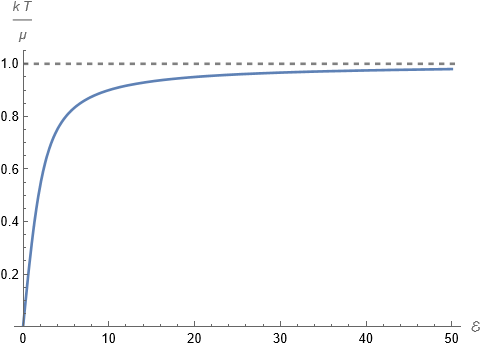
\includegraphics[width=0.6\linewidth]{grafico1}
	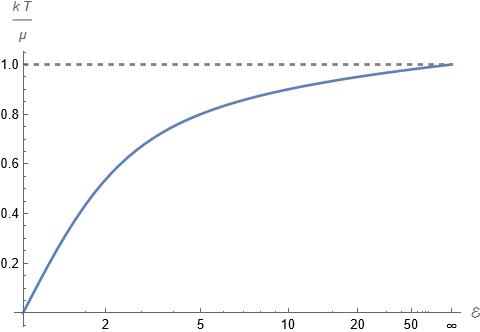
\includegraphics[width=0.6\linewidth]{grafico2}
	\label{2.16_graficos}
\end{figure}

NOTA: Se usó Wolfram Mathematica para las derivadas y los gráficos.

% % % % % % % % % % % % % % % % % % % % % % % % % % % % % % % % % % % % % % % % % % % % % % % % % % % % % %
\section{Problema 2.17}
In Chapter 14 we shall derive an approximate partition function for a dense gas, which is of the form
\begin{equation}
	Q(N, V, T)=\frac{1}{N!}\left(\frac{2 \pi m k T}{h^2}\right)^{3 N / 2}(V-N b)^N e^{a N^2 / V k T}
	\label{2.17_Q}
\end{equation}
where $a$ and $b$ are constants that are given in terms of molecular parameters. Calculate the equation of state from this partition function. What equation of state is this? Calculate the thermodynamic energy and the heat capacity and compare it to Problem 1-30.
\\

\textbf{Respuesta:}
Introduciendo la ec. \ref{2.17_Q} en la relación
\begin{equation}
	p = k T \deriv{\ln Q}{V}{T,N}\label{p_QVTN}
\end{equation}
obtenemos
\begin{equation}
	p =\frac{N k T}{V - N b}-\frac{a N^2}{V^2}
\end{equation}
La cual coincide con la ecuación de de Van der Waals (ec. \ref{VanDerWaals}).\qed

Luego, para la energía y la capacidad calórica, aplicamos las ecs. \ref{U_QTVN} y \ref{CV_UTVN}:
\begin{align}
	U &= k T^2 \deriv{\ln Q}{T}{V,N}\nonumber\\
	U &= \frac{3 N k T}{2} - \frac{a N^2}{V}
\end{align}
\qed

\begin{align}
	C_V &= \deriv{U}{T}{V,N}\nonumber\\
	C_V &= \frac{3 N k}{2}	
\end{align}
\qed

NOTA: Se usó Wolfram Mathematica para las derivadas.

% % % % % % % % % % % % % % % % % % % % % % % % % % % % % % % % % % % % % % % % % % % % % % % % % % % % % %
\section{Problema 3.4}
State and use Euler's theorem to show
\begin{equation}
	p=k T\left(\frac{\partial \ln \Xi}{\partial V}\right)_{\mu, T}=k T \frac{\ln \Xi}{V}
\end{equation}
\\

\textbf{Respuesta:}
El teorema de Euler dice que para cualquier función \(f\) homogénea de orden \(n\), es decir, que cumpla con
\begin{equation*}
	f(\lambda x_1,\lambda x_2,\ldots,\lambda x_N) = \lambda^n f(x_1,x_2,\ldots,x_N)
\end{equation*}
entonces
\begin{equation}
	n f(x_1,x_2,\ldots,x_N) = x_1 \frac{\partial f}{\partial x_1} + x_2 \frac{\partial f}{\partial x_2} + \cdots + x_N \frac{\partial f}{\partial x_N}\label{Euler}
\end{equation}
Si consideramos un sistema de volumen \(V\) en equilibrio con un reservorio, y aumentamos el volumen por un factor \(\lambda\), manteniendo fijos \(\mu, T\), tendremos, equivalentemente, \(\lambda\) copias idénticas e independientes una al lado de la otra.
\begin{figure}[h!]
	\centering
	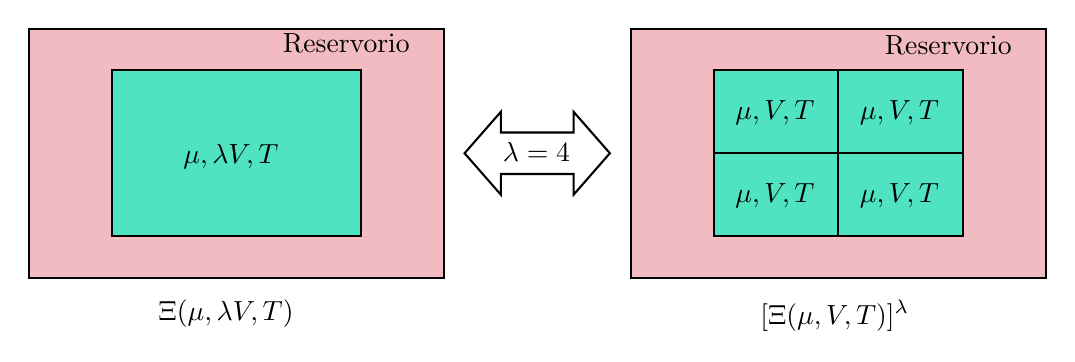
\begin{tikzpicture}[x=0.75pt,y=0.75pt,yscale=-1,xscale=1]
		%uncomment if require: \path (0,300); %set diagram left start at 0, and has height of 300
		
		%Shape: Rectangle [id:dp04643399035683926] 
		\draw  [fill={rgb, 255:red, 208; green, 2; blue, 27 }  ,fill opacity=0.27 ] (20,20) -- (220,20) -- (220,140) -- (20,140) -- cycle ;
		%Shape: Rectangle [id:dp05712486709081854] 
		\draw  [fill={rgb, 255:red, 80; green, 227; blue, 194 }  ,fill opacity=1 ] (60,40) -- (180,40) -- (180,120) -- (60,120) -- cycle ;
		%Shape: Rectangle [id:dp812030185769934] 
		\draw  [fill={rgb, 255:red, 208; green, 2; blue, 27 }  ,fill opacity=0.27 ] (310,20) -- (510,20) -- (510,140) -- (310,140) -- cycle ;
		%Shape: Rectangle [id:dp6459894702909416] 
		\draw  [fill={rgb, 255:red, 80; green, 227; blue, 194 }  ,fill opacity=1 ] (350,40) -- (410,40) -- (410,80) -- (350,80) -- cycle ;
		%Shape: Rectangle [id:dp1790662573806695] 
		\draw  [fill={rgb, 255:red, 80; green, 227; blue, 194 }  ,fill opacity=1 ] (350,80) -- (410,80) -- (410,120) -- (350,120) -- cycle ;
		%Shape: Rectangle [id:dp8411636418864974] 
		\draw  [fill={rgb, 255:red, 80; green, 227; blue, 194 }  ,fill opacity=1 ] (410,40) -- (470,40) -- (470,80) -- (410,80) -- cycle ;
		%Shape: Rectangle [id:dp8708466031889306] 
		\draw  [fill={rgb, 255:red, 80; green, 227; blue, 194 }  ,fill opacity=1 ] (410,80) -- (470,80) -- (470,120) -- (410,120) -- cycle ;
		%Left Right Arrow [id:dp8925469394918272] 
		\draw   (230,80) -- (247.5,60) -- (247.5,70) -- (282.5,70) -- (282.5,60) -- (300,80) -- (282.5,100) -- (282.5,90) -- (247.5,90) -- (247.5,100) -- cycle ;
		
		% Text Node
		\draw (141,21) node [anchor=north west][inner sep=0.75pt]   [align=left] {Reservorio};
		% Text Node
		\draw (431,22) node [anchor=north west][inner sep=0.75pt]   [align=left] {Reservorio};
		% Text Node
		\draw (93,74) node [anchor=north west][inner sep=0.75pt]   [align=left] {$\displaystyle \mu ,\lambda V,T$};
		% Text Node
		\draw (359,53) node [anchor=north west][inner sep=0.75pt]   [align=left] {$\displaystyle \mu ,V,T$};
		% Text Node
		\draw (359,93) node [anchor=north west][inner sep=0.75pt]   [align=left] {$\displaystyle \mu ,V,T$};
		% Text Node
		\draw (419,93) node [anchor=north west][inner sep=0.75pt]   [align=left] {$\displaystyle \mu ,V,T$};
		% Text Node
		\draw (419,53) node [anchor=north west][inner sep=0.75pt]   [align=left] {$\displaystyle \mu ,V,T$};
		% Text Node
		\draw (81,149) node [anchor=north west][inner sep=0.75pt]   [align=left] {$\displaystyle \Xi ( \mu ,\lambda V,T)$};
		% Text Node
		\draw (371,149) node [anchor=north west][inner sep=0.75pt]   [align=left] {$\displaystyle [ \Xi ( \mu ,V,T)]^{\lambda }$};
		% Text Node
		\draw (247,73) node [anchor=north west][inner sep=0.75pt]   [align=left] {$\displaystyle \lambda =4$};
	\end{tikzpicture}
\end{figure}
Escalar el sistema de esta forma nos deja con una función de partición igual al producto de las funciones de los subsistemas, es decir:
\begin{equation}
	\Xi(\mu,\lambda V,T) = \left[\Xi(\mu,V,T)\right]\lambda
\end{equation}
Luego:
\begin{equation}
	\ln \Xi(\mu,\lambda V,T) = \lambda\ln\Xi(\mu,V,T)
\end{equation}
Por lo que \(\ln \Xi\) es homogénea de orden 1 respecto a \(V\), mientras que \(\mu,T\) no escalan por ser intensivas.
Entonces, siguiendo la ec. \ref{Euler}:
\begin{align}
	\ln \Xi(\mu,V,T) &= V \deriv{\ln\Xi}{V}{\mu,T}\nonumber\\
	\Rightarrow\frac{\ln\Xi}{V} &= \deriv{\ln\Xi}{V}{\mu,T}
\end{align}
Aplicando la relación:
\begin{equation}
	p = k T\frac{\ln\Xi}{V}
\end{equation}
Obtenemos finalmente:
\begin{equation}
	p = k T\frac{\ln\Xi}{V} = k T \deriv{\ln\Xi}{V}{\mu,T}
\end{equation}
\qed

% % % % % % % % % % % % % % % % % % % % % % % % % % % % % % % % % % % % % % % % % % % % % % % % % % % % % %
\section{Problema 3.5}
Show that the entropy given by
\begin{equation}
	S = \frac{\bar{E}}{T} - \frac{\bar{N}\mu}{T} + k \ln\Xi\label{S_T0}
\end{equation}
goes to zero as \(T\) goes to zero.
\\

\textbf{Respuesta:}
Considerando
\begin{equation}
	\Xi = \sum_{N,j} e^{-(E_{N,j} - N \mu)/kT}\label{Xi}
\end{equation}
Definiendo
\begin{equation}
	G_{N,j} \equiv E_{N,j} - N \mu\label{3.5_G}
\end{equation}
Y tomando el límite \(T\rightarrow 0 \)
\begin{equation*}
	\lim_{T\rightarrow 0}\Xi = \sum_{N,j} e^{-G_{N,j}/kT}
\end{equation*}
Tendremos que este estará dominado por el valor mínimo de \(G_{N,j}\), o el \textit{ground state}:
\begin{equation}
	G_0 = \min \left(G_{N,j}\right)\label{3.5_G0}
\end{equation}
Factorizando:
\begin{align*}
	\lim_{T\rightarrow 0}\Xi &= e^{-G_0/kT} \left[ \sum_{N,j} e^{-(G_{N,j} - G_0)/kT} \right]\\
	&= e^{-G_0/kT} \left[ \sum_{G_{N,j} = G_0} \underbrace{e^{-(G_0 - G_0)/kT}}_{1} + \sum_{G_{N,j} > G_0} e^{-(G_{N,j} - G_0)/kT} \right]\\
	&= e^{-G_0/kT} \left[ g_0 + \sum_{G_{N,j} > G_0} e^{-(G_{N,j} - G_0)/kT} \right]
\end{align*}
Donde \(g_0\) es la degeneración de \(G_0\), es decir, la cantidad de estados que comparten este estado de energía. Evaluando el límite tendremos que los términos de orden superior se anularán:
\begin{equation}
	\Xi \approx e^{-G_0/kT} \left[ g_0 + 0 \right] = g_0 e^{-G_0/kT}\label{3.5_Xi_T0}
\end{equation}
Luego,
\begin{equation}
	\ln\Xi \approx\ln g_0 - \dfrac{G_0}{kT} 
\end{equation}
Reemplazando esto en la ec. \ref{S_T0}:
\begin{align*}
	S &\approx \frac{\bar{E} - \bar{N}\mu}{T} + k \left(\ln g_0 - \dfrac{G_0}{kT} \right)\\
	&\approx \frac{\bar{E} - \bar{N}\mu}{T} + k \ln g_0 - \dfrac{G_0}{T}
\end{align*}
Pero tendremos que, cuando \(T\rightarrow 0\), los valores promedio \(\bar{E}\) y \(\bar{N}\) tienden a los correspondientes al \textit{ground state}, por ser este el estado más probable. Por lo que, usando la definición de \ref{3.5_G}:
\begin{equation}
	\lim_{T\rightarrow 0} \left(\bar{E} - \bar{N}\mu\right) \approx G_0
\end{equation}
Luego
\begin{align}
	S &\approx \frac{G_0}{T} + k \ln g_0 - \dfrac{G_0}{T}\nonumber\\
	S &\approx k\ln g_0
\end{align}
Finalmente, la Tercera Ley de la Termodinámica nos dice que, para la mayoría de los sistemas cristalinos, solo existirá un sistema en el estado base:
\begin{equation}
	g_0 = 1
\end{equation}
Por lo que:
\begin{equation}
	S \approx k\ln 1 = 0
\end{equation}
\qed
\end{document}